\documentclass[11pt]{article}
\usepackage{geometry}                
\geometry{letterpaper}
\usepackage[]{graphicx}
\usepackage{amssymb}
\usepackage{enumitem}
\usepackage{hyperref}
\usepackage{amsmath}
\usepackage{multicol}
\usepackage{braket}
\usepackage{pdfpages}


\begin{document}

\begin{center}
    {\LARGE Python Implementation of Stabilizer Algorithms }
\vspace{2mm}
{\large \\ Patrick Rall, Iskren Vankov - \today}
\end{center}

% useful for multicolumn figures
\newenvironment{Figure}
  {\par\medskip\noindent\minipage{\linewidth}}
  {\endminipage\par\medskip}


\subsection*{Progress over break}
\begin{itemize}
    \item Implement \textsc{ExponentialSum}
    \item More testing: \textbf{Code is definitely buggy!}
\end{itemize}

\subsection*{Questions}
\begin{itemize}
    \item What is wrong with the code below?
    \item \textbf{Unit tests: What tests can we perform to validate the implementations?}
    \item How to decompose $W(\mathcal{K},q)$ into integers $p,m,\epsilon$? Detailed in [15]?
\end{itemize}

\subsection*{Goals for next week}
\begin{itemize}
    \item \textit{Patrick}: Implement the remaining routines: \textsc{InnerProduct} and \textsc{MeasurePauli}
    \item \textit{Patrick}: Implement the main quantum circuit simulator
    \item \textit{Patrick}: Debug code, implement unit tests
    \item \textit{Iskren}: Identify C++ linalg libraries, review for threading support
    \item \textit{Iskren}: Review, understand, and debug code below
\end{itemize}

\clearpage

\begin{center}
    {\Large Some random stabilizer states }
\end{center}

\begin{multicols}{3}
\begin{verbatim}
States with n = 2

State 1:
00 (1+0j)
01 (1+0j)
10 (1+0j)
11 (1+0j)
Norm: 4.0

State 2:
00 (1+0j)
01 (1+0j)
10 (1+0j)
11 (1+0j)
Norm: 4.0

State 3:
00 (1+0j)
01 (1+0j)
10 (1+0j)
11 (1+0j)
Norm: 4.0

State 4:
00 (1+0j)
01 (1+0j)
10 (1+0j)
11 (1+0j)
Norm: 4.0

State 5:
00 (1+0j)
01 (1+0j)
10 (1+0j)
11 (1+0j)
Norm: 4.0
\end{verbatim}
\vfill
\columnbreak
\begin{verbatim}
States with n = 3

State 1:
000 (1+0j)
001 (1+0j)
010 (1+0j)
011 (1+0j)
100 (1+0j)
101 (1+0j)
110 (1+0j)
111 (1+0j)
Norm: 8.0

State 2:
011 (0.5+0.5j)
111 (-0.5-0.5j)
Norm: 1.0

State 3:
010 (0.707+0j)
110 (-0-0.707j)
Norm: 1.0

State 4:
010 0.707j
110 (-0.707+0j)
Norm: 1.0

State 5:
010 (-0.5+0.5j)
110 (0.5+0.5j)
Norm: 1.0
\end{verbatim}
\vfill
\columnbreak
\begin{verbatim}
States with n = 4

State 1:
0110 (-0.5+0.5j)
1110 (-0.5+0.5j)
Norm: 1.0

State 2:
0000 (0.354+0.354j)
0100 (-0.354+0.354j)
1000 (-0.354-0.354j)
1100 (0.354-0.354j)
Norm: 1.0

State 3:
0001 (0.354-0.354j)
0101 (0.354-0.354j)
1001 (0.354+0.354j)
1101 (-0.354-0.354j)
Norm: 1.0

State 4:
0000 (-0-0.5j)
0100 (-0-0.5j)
1000 (0.5+0j)
1100 (0.5+0j)
Norm: 1.0

State 5:
0001 (-0.354+0.354j)
0101 (0.354-0.354j)
1101 (0.354-0.354j)
Norm: 0.75
\end{verbatim}
\end{multicols}

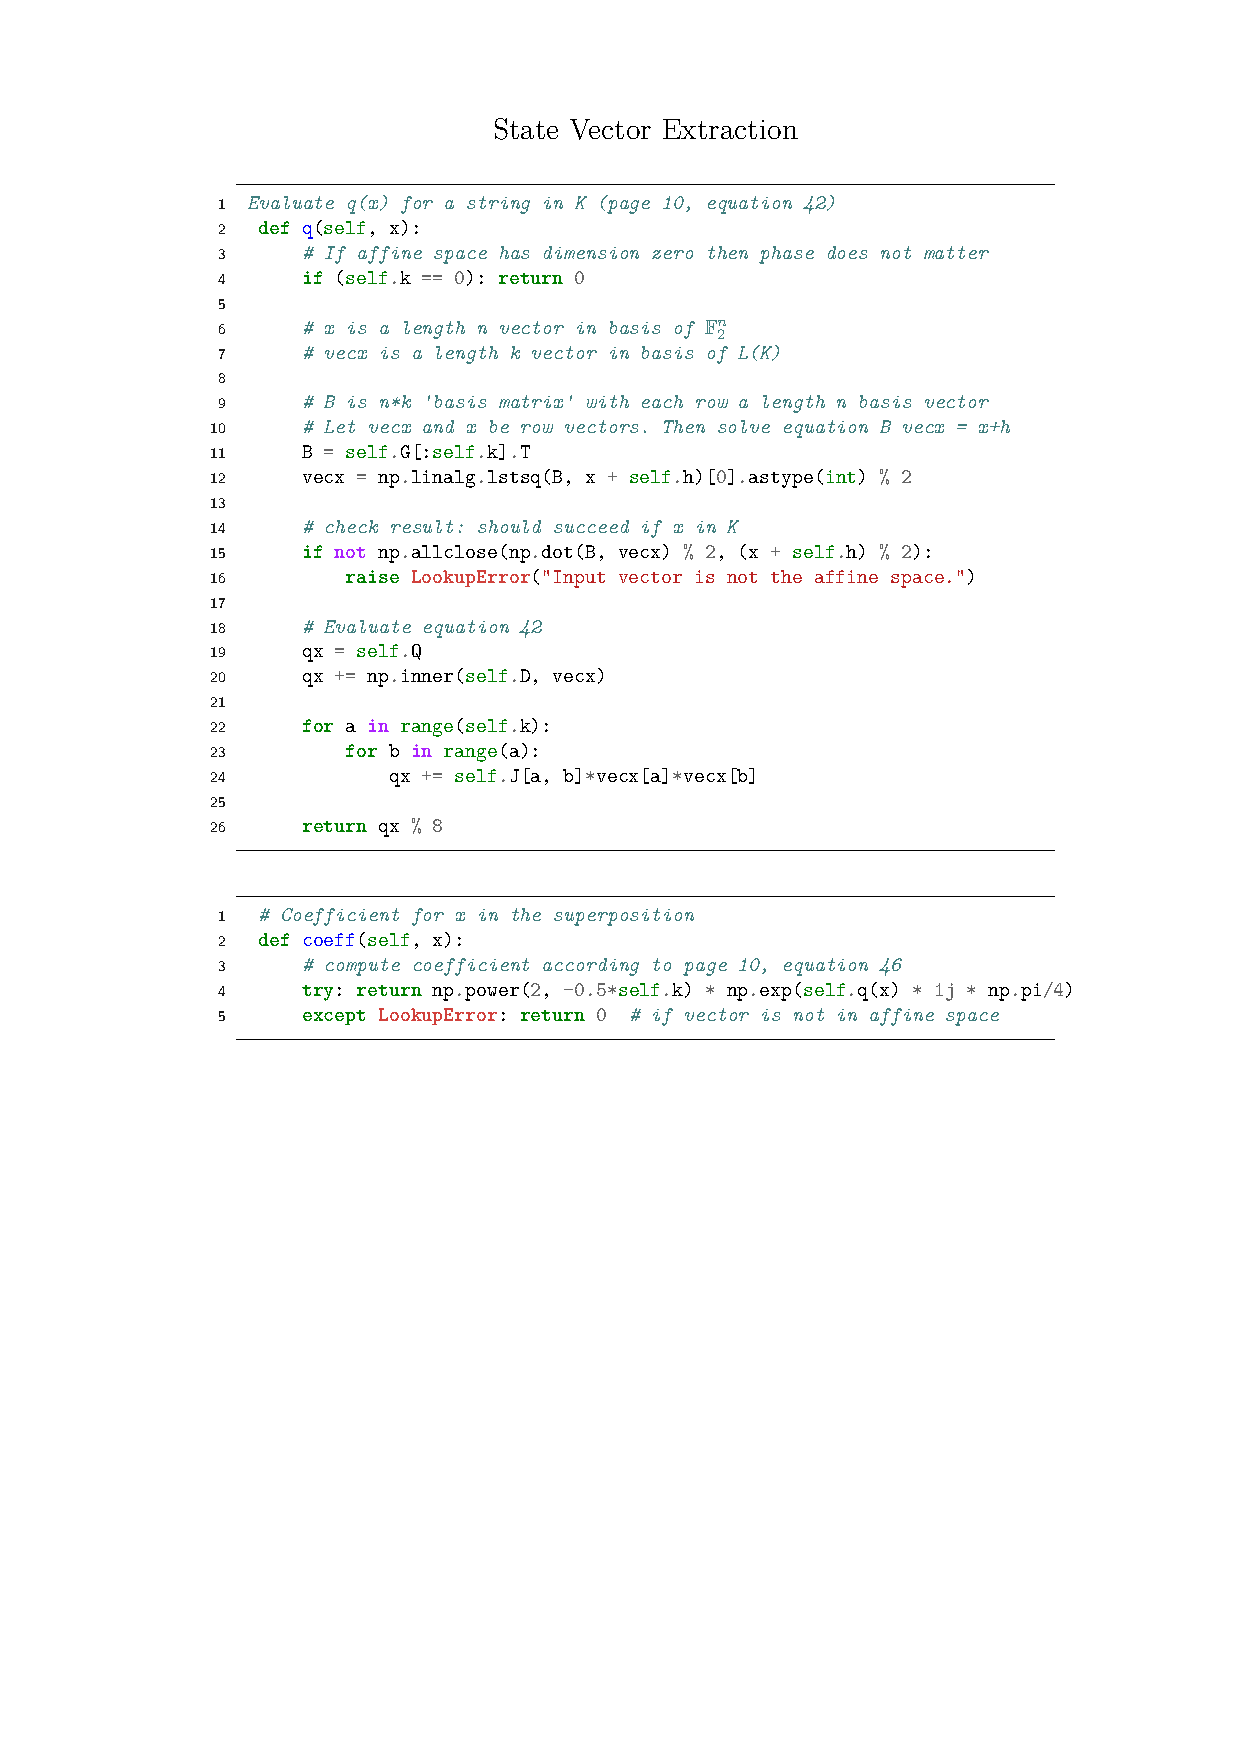
\includepdf[pages=-]{mar28-figs/extract.pdf}
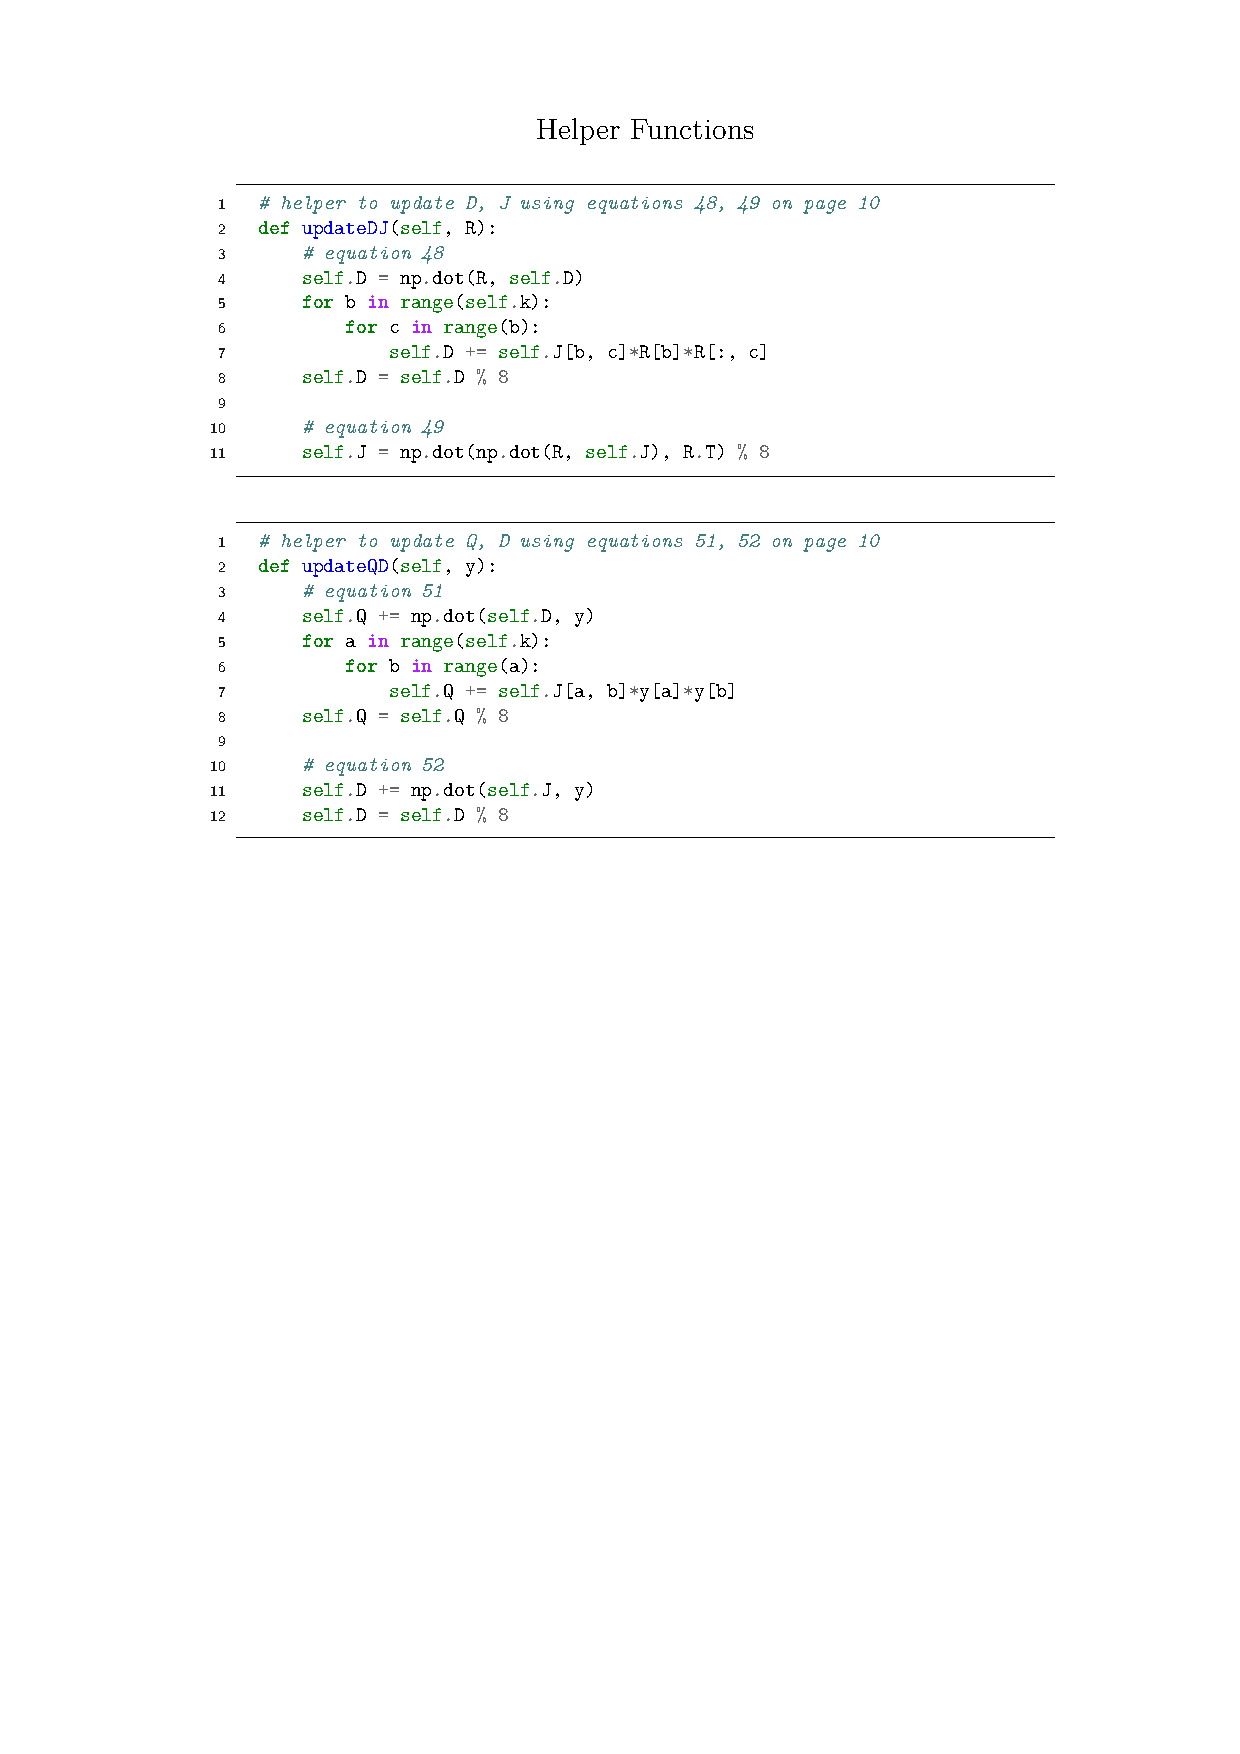
\includepdf[pages=-]{mar28-figs/helpers.pdf}
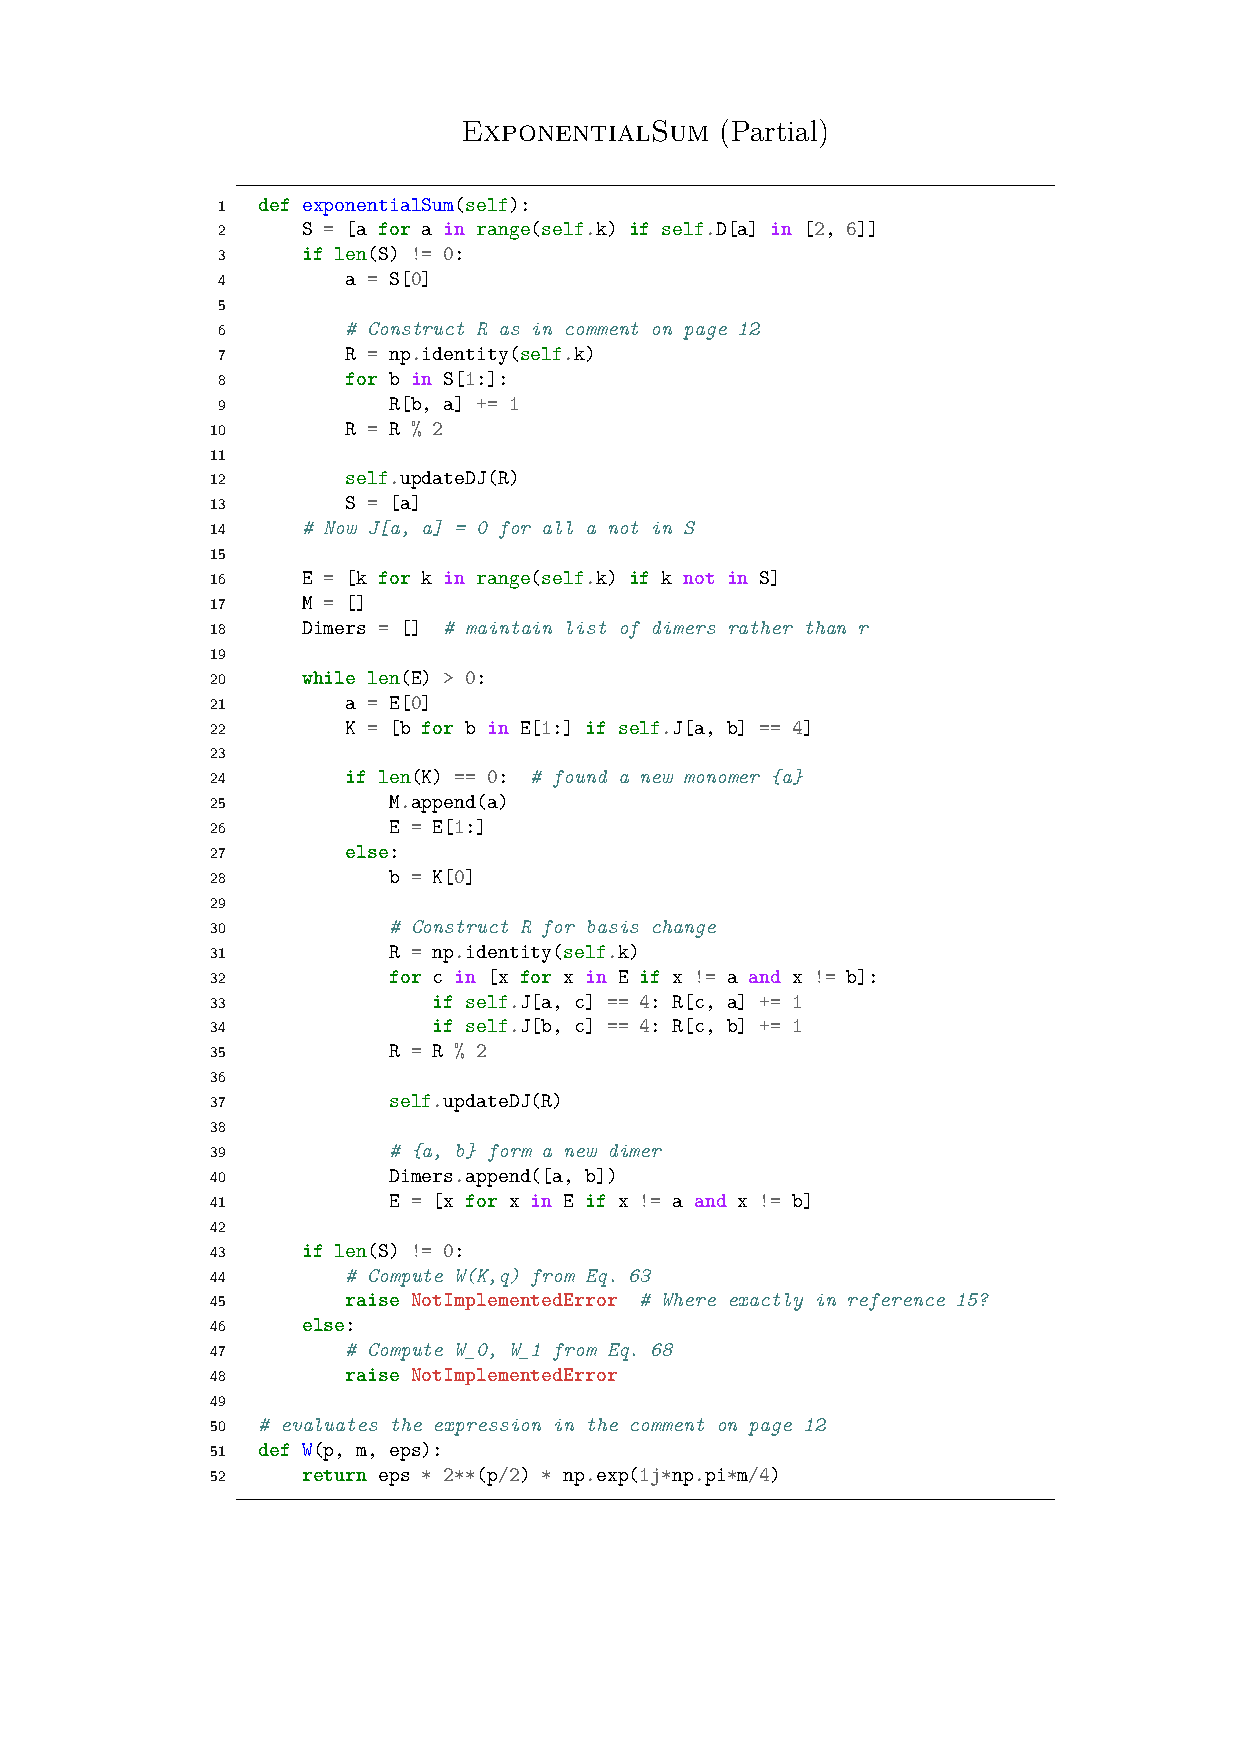
\includepdf[pages=-]{mar28-figs/expSum.pdf}
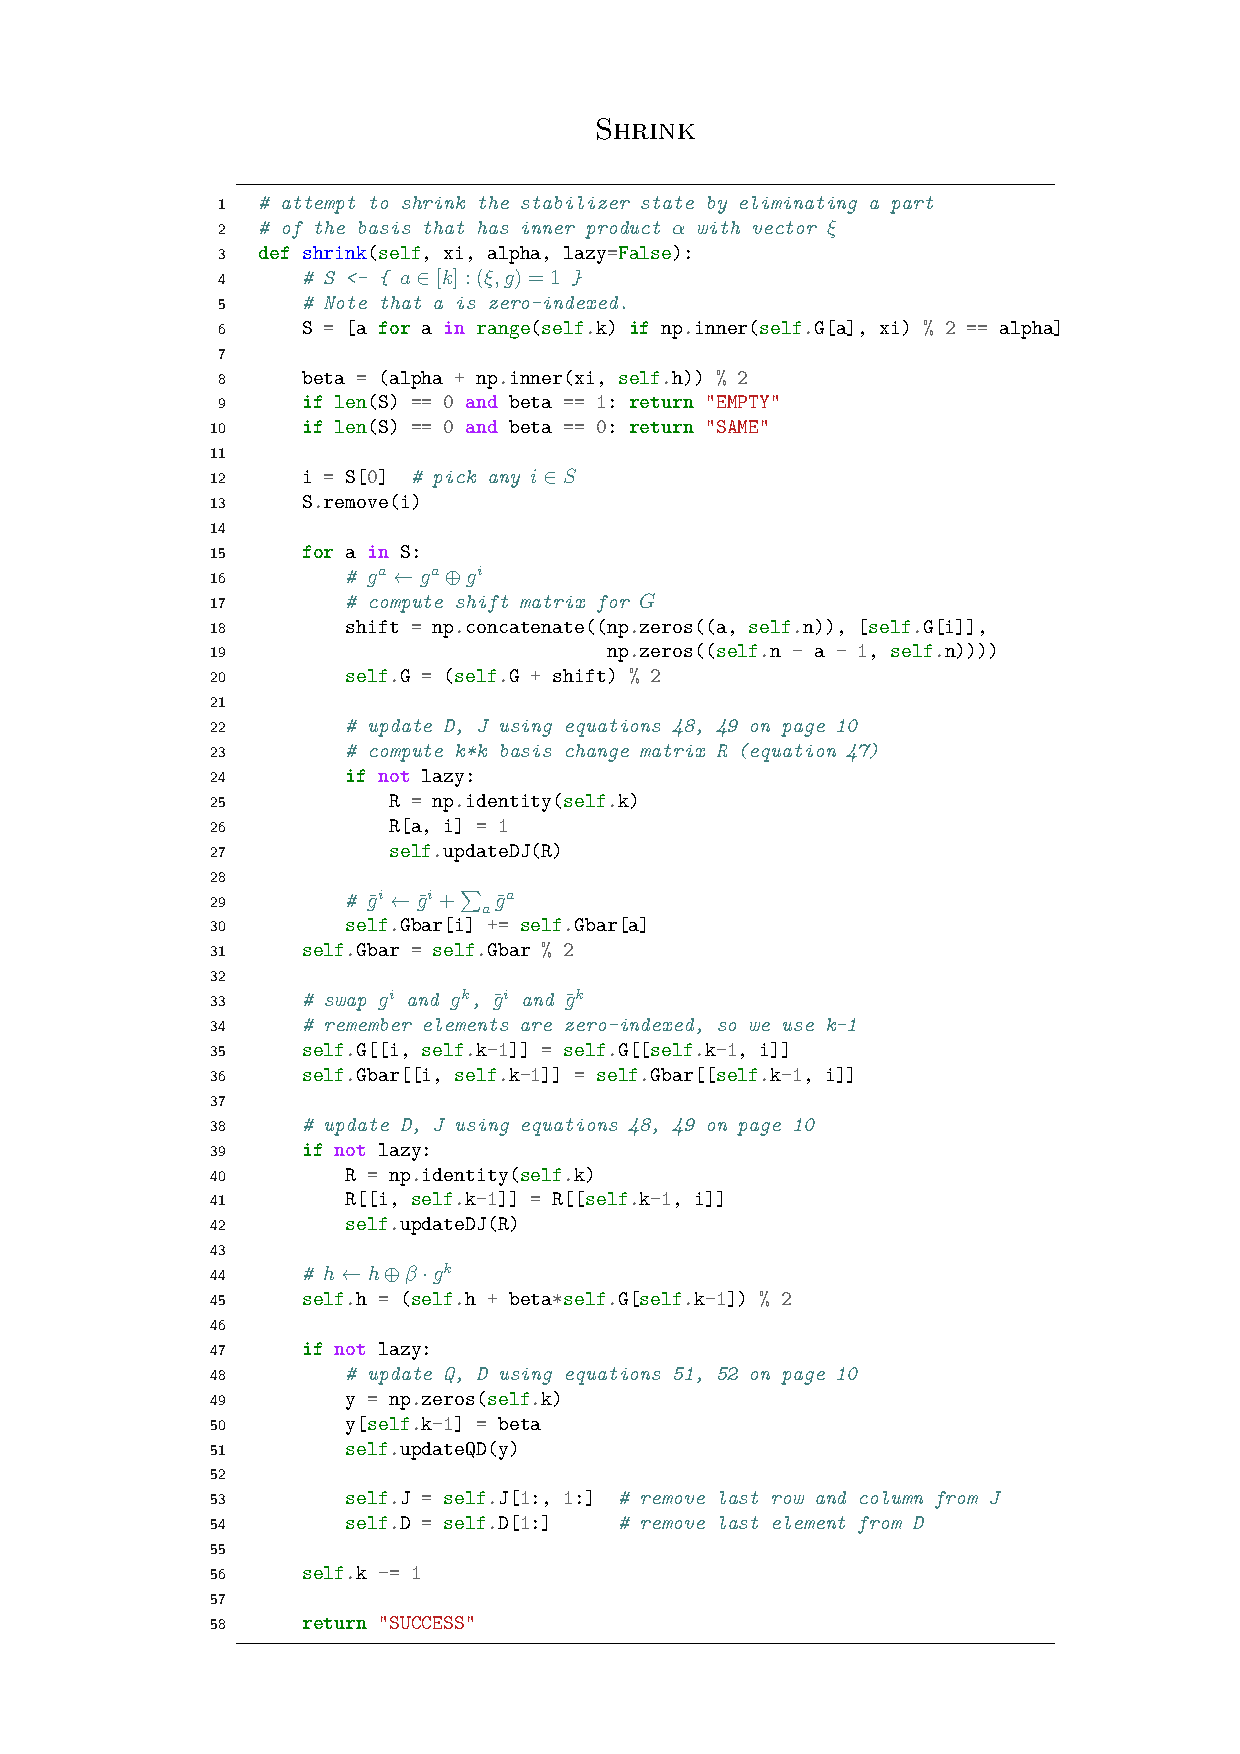
\includepdf[pages=-]{mar28-figs/shrink.pdf}
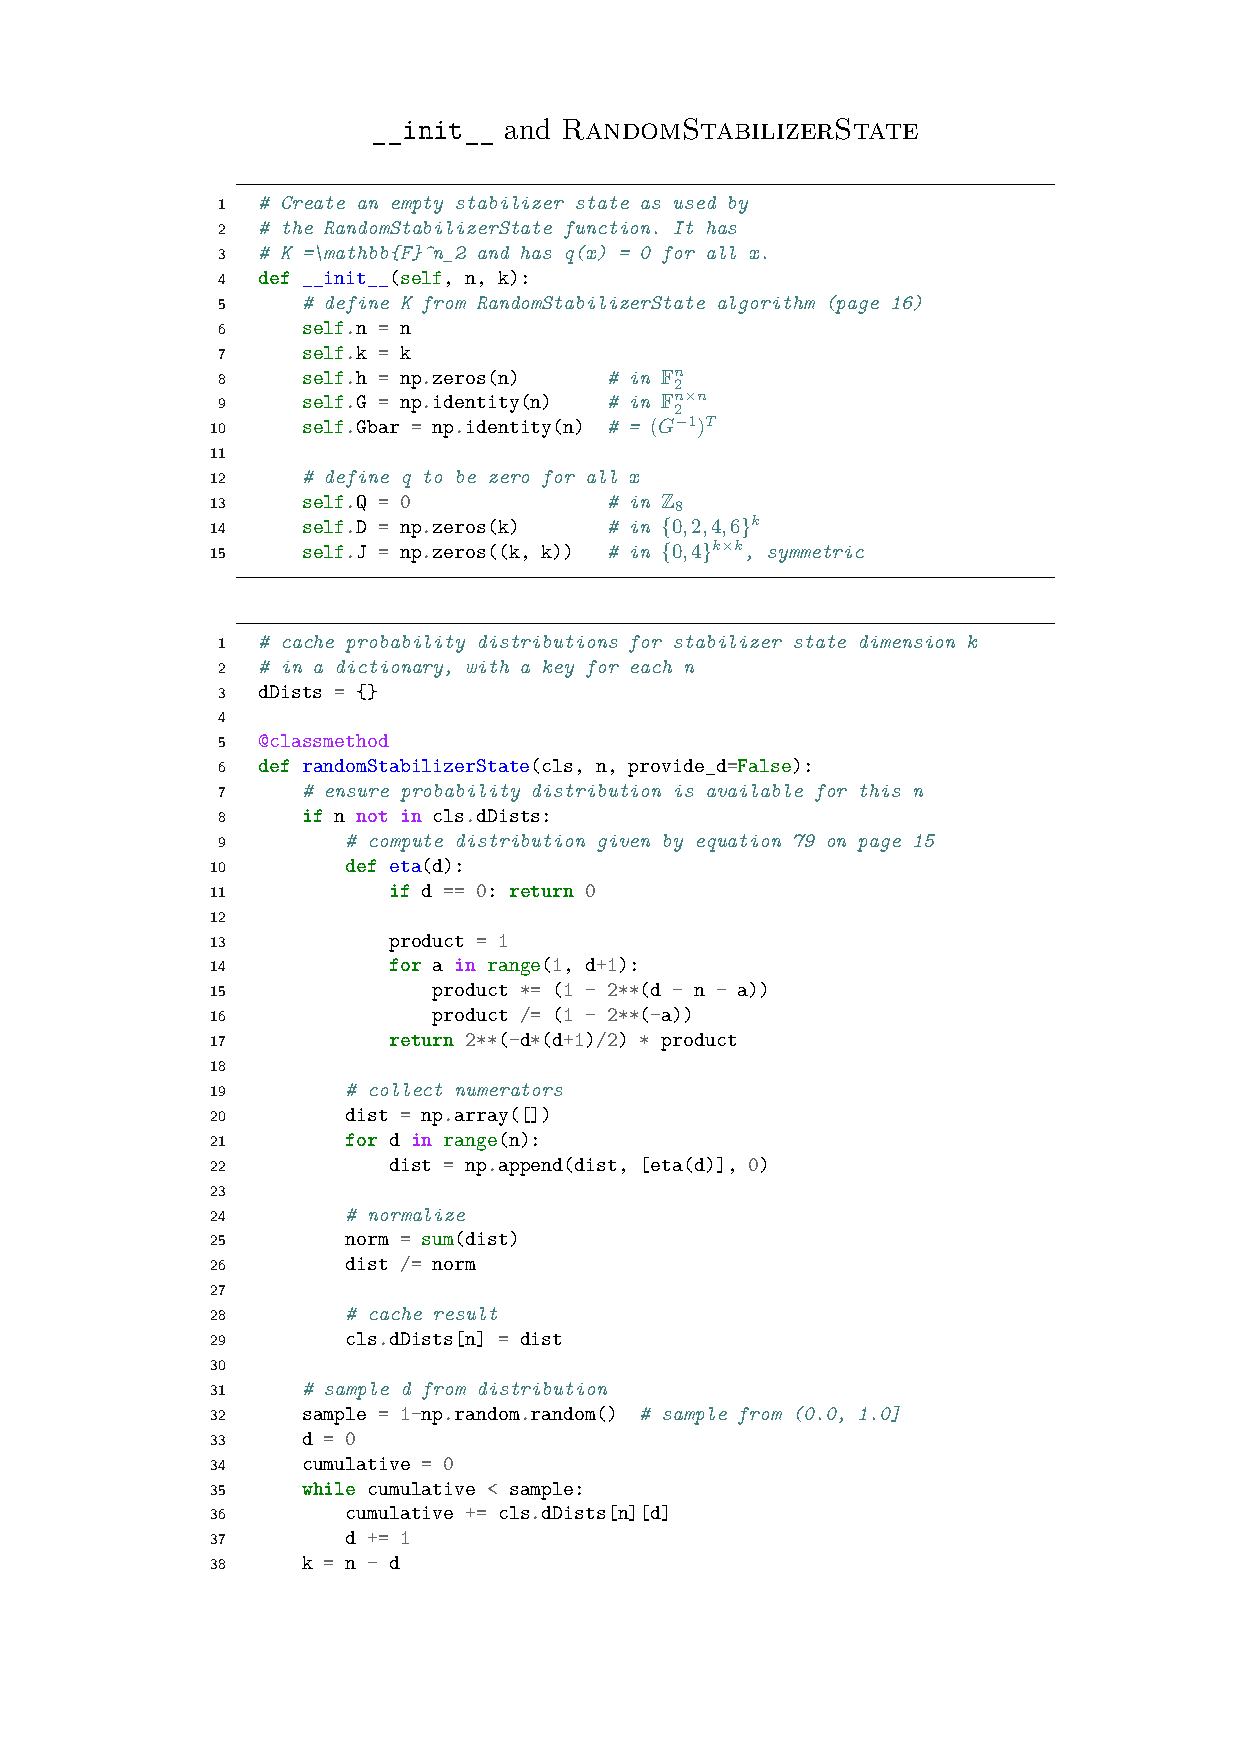
\includepdf[pages=-]{mar28-figs/random.pdf}

\end{document}

